\section{Project Dependent Preparations} \label{sec:project-prep}

This section summarises the project-specific preparations completed or in progress at the time of this report. The focus for Thesis~A is on building a minimal but functional vision pipeline using ArUco fiducials on real images, and developing an initial CAD model of the free-floating docking station. These activities provide early evidence that the proposed methodology is practical and that the broader Thesis~B/C timeline is achievable.

\subsection{Setting up Software Environment}

To support the planned vision-based docking system, the following software tools and libraries have been set up:

\begin{itemize}
    \item \textbf{Python and OpenCV:} A Python~3 environment has been configured with the OpenCV and \texttt{opencv-contrib} libraries for image capture, pre-processing and ArUco marker detection. Basic camera access and image display have been verified on the target machine.
    \item \textbf{ArUco pose estimation tools:} The OpenCV ArUco module has been installed and a small calibration and pose-estimation pipeline has been developed. This includes camera calibration using a chessboard pattern, marker detection, and Perspective-\emph{n}-Point (PnP) pose estimation with visual overlays on the image.
    \item \textbf{ROS~2 Humble workspace:} A ROS~2 Humble workspace has been created to host the future ROV control stack. Within this workspace, a prototype ``vision node'' package has been started, intended to wrap the ArUco pose-estimation pipeline and publish the estimated dock pose as a ROS~2 message for later use by the controller.
    \item \textbf{CAD tooling:} A parametric CAD package (e.g.\ SolidWorks / Fusion~360) has been selected for modelling the docking station, and an initial project structure has been created for the dock geometry, mounting points and marker/light locations.
    \item \textbf{Version control:} A private Git repository has been created to store Python scripts, ROS~2 packages, CAD files and experimental configuration. This enables reproducibility and incremental development across Thesis~B and~C.
\end{itemize}

\subsection{Preliminary ArUco Pose Estimation Prototype}

As an initial proof-of-concept, a basic ArUco-based pose estimation pipeline has been implemented using real camera images. The goal at this stage is not full docking, but to verify that:

\begin{enumerate}
    \item ArUco markers can be reliably detected under underwater-like lighting conditions, and
    \item the resulting Perspective-\emph{n}-Point (PnP) pose estimates behave sensibly as the camera moves.
\end{enumerate}

The prototype currently consists of two main components. First, a standalone Python calibration script is used to estimate the intrinsic parameters and distortion coefficients of the camera from a set of checkerboard images. This script runs offline (outside ROS~2) and outputs a calibration file (\texttt{camera\_calib.npz}) containing the camera matrix and distortion coefficients that are later loaded by the vision node at runtime.

\begin{figure}[H]
    \centering
    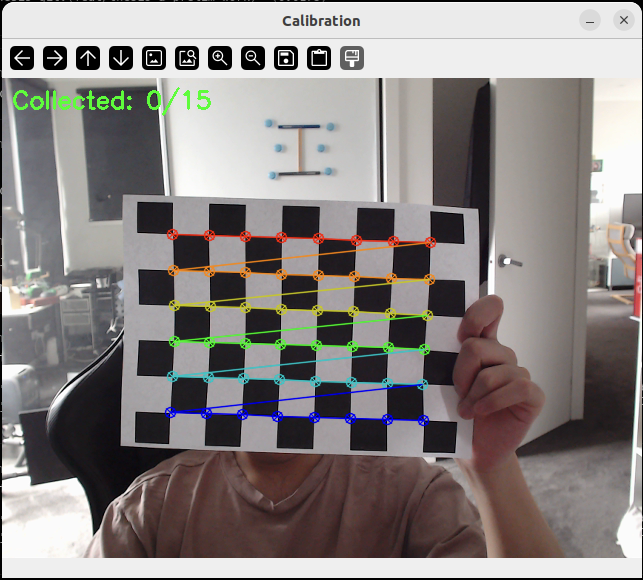
\includegraphics[width=0.5\textwidth]{Figures/camera-calibration.png}
    \caption{Example of sampling frames used for camera calibration with a chessboard pattern.}
    \label{fig:aruco-prototype-frame}
\end{figure}

Second, the core ArUco-based detection and pose estimation pipeline has been implemented as a ROS~2 Humble node. This node subscribes to a camera image topic (e.g.\ \texttt{/camera/image\_raw}), applies the pre-computed calibration, detects ArUco markers in each frame, and computes their 6-DoF pose using OpenCV's PnP solver. Detection overlays (marker borders and coordinate axes) are rendered into a debug image stream, and the estimated translation and orientation of the marker are published as a \texttt{PoseStamped} message on a dedicated topic (e.g.\ \texttt{/dock\_pose}). A simplified view of the current node setup for this prototype is shown in Figure~\ref{fig:ros2-vision-node}.

\begin{figure}[H]
    \centering
    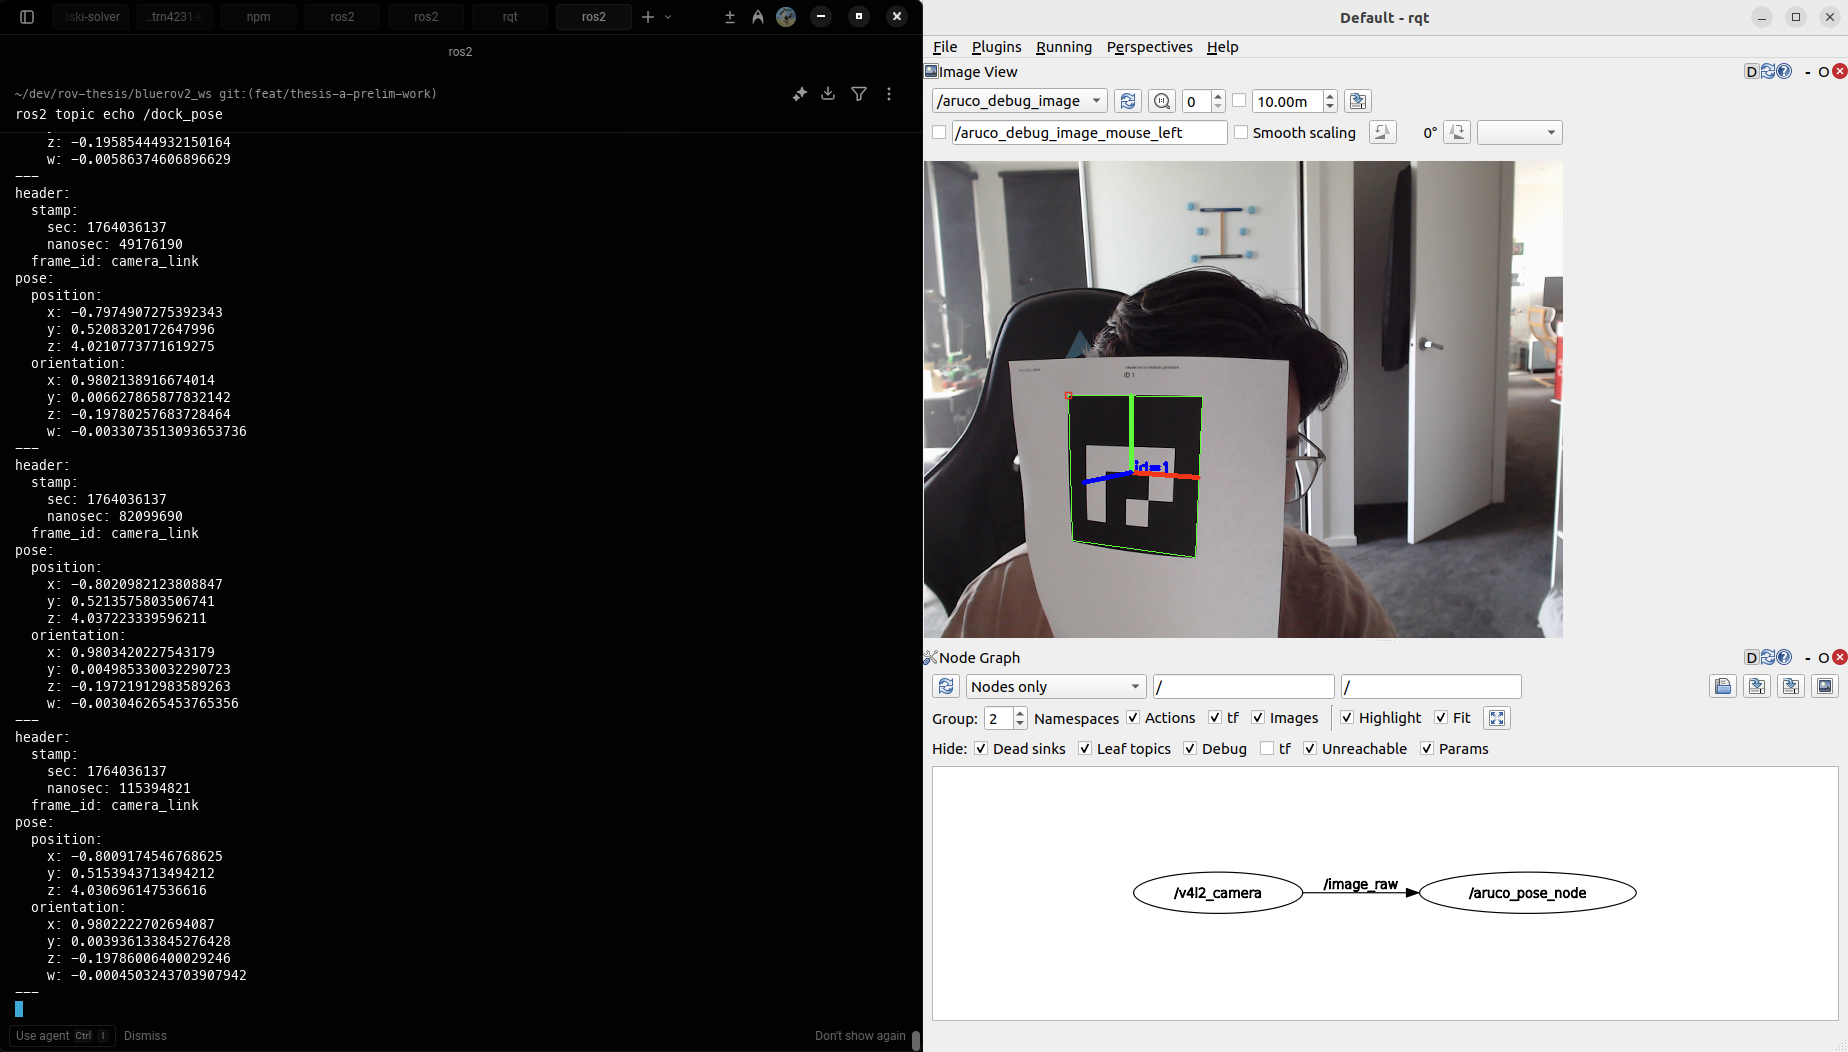
\includegraphics[width=0.7\textwidth]{Figures/aruco-demo.png}
    \caption{Initial ROS~2 Humble vision node prototype: the ArUco-based pose-estimation node subscribes to camera images, applies calibration and publishes an estimated dock pose topic for use by control and logging modules.}
    \label{fig:ros2-vision-node}
\end{figure}

These preliminary results demonstrate that marker-based pose estimation can be implemented and integrated into the ROS~2 environment on the target hardware. In subsequent thesis stages, this prototype will be extended to handle multiple markers, underwater imagery, turbidity-aware pre-processing and tighter coupling with the ROV's navigation and control stack.

\subsection{Initial Docking Station CAD Model}
An initial concept CAD model of the free-floating docking station has been developed, focusing on:
\begin{itemize}
    \item \textbf{Marker placement:} Locations for ArUco fiducials arranged to maximise visibility from multiple approach angles, considering occlusions and perspective distortion.
    \item \textbf{Active lighting:} Integration points for LED beacons to provide long-range guidance in low-visibility conditions.
\end{itemize}

\noindent The dock station is designed to be suspended from a floating platform (see Figures~\ref{fig:docking-station-cad} and \ref{fig:docking-station-cad-with-rov}).

\begin{figure}[H]
    \centering
    \begin{subfigure}[b]{0.48\textwidth}
        \centering
        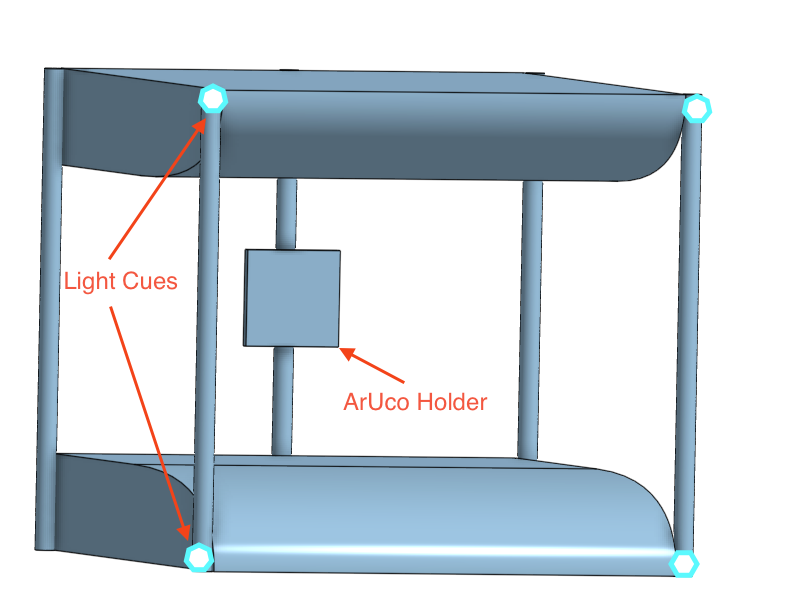
\includegraphics[width=\textwidth]{Figures/custom-dock-station.png}
        \caption{}
        \label{fig:docking-station-cad}
    \end{subfigure}\hfill
    \begin{subfigure}[b]{0.48\textwidth}
        \centering
        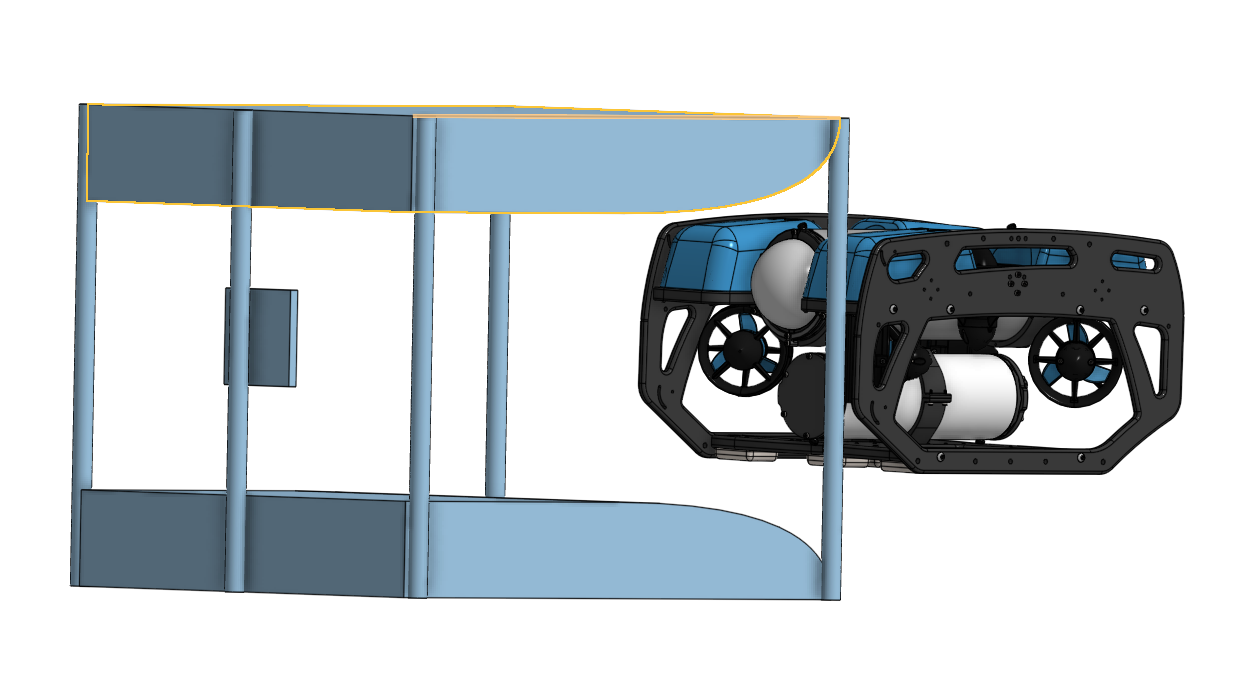
\includegraphics[width=\textwidth]{Figures/custom-dock-station-with-rov.png}
        \caption{}
        \label{fig:docking-station-cad-with-rov}
    \end{subfigure}
    \caption{Concept CAD views: (a) docking station with marker and LED placements; (b) docking station with BlueROV2 for scale.}
    \label{fig:docking-station-combined}
\end{figure}